% =====================================================================
%  chunks/ch03a.tex —— 原书 p.40 中部–p.46（PDF 47 中部–53）
%  第 3 章章标题 + §1 单纯复形
%  块止于 p.46 末句「…经标准重分后仍为单纯复形。」；p.47 顶端括注归 ch03b。
% =====================================================================
% [原文 p.40]
\chapter[单纯复形与 CW 复形。同调与上同调。它们与同伦论的关系。障碍]{单纯复形与 $CW$ 复形。同调与上同调。它们与同伦论的关系。障碍}

\section{单纯复形}
\takeaway{单纯复形是满足「含面」与「交于公共面」两条公理的单形族，$n$ 维单形是 $\R^n$ 中 $n+1$ 个一般位置的顶点的凸包。核心工具是重心重分与 Euler--Poincaré 示性数 $\chi(K)=\sum_j(-1)^j\gamma_j$，核心概念是组合等价与单纯逼近定理。}

单纯复形（最早由 Poincaré 引入）为同调群与上同调群的定义、以及为研究它们的形式性质，提供了最干净、也最便于严格处理的途径，这一点我们很快就会看到；不过要具体计算这些群，它并不方便。
% [原文 p.41]
我们把 $n$ 维单形 $\sigma_n$ 定义为 $\R^n$ 中任意 $n+1$ 个不位于任何 $(n-1)$ 维超平面内的点 $\alpha_0,\dots,\alpha_n$ 的凸包（见图 3.1）。于是 $\sigma^n=(\alpha_0,\dots,\alpha_n)$ 的点是顶点 $\alpha_0,\dots,\alpha_n$（看作 $n$ 维向量）的如下形式的线性组合：
\begin{equation}
  x\in\sigma^n,\qquad x=\sum_{j=0}^{n}x^j\alpha_j,\qquad
  \sum_{j=0}^{n}x^j=1,\qquad x^j\ge0. \tag{1.1}
\end{equation}
% [Tutor Note: 原书 p.41 这一句先把 $n$ 维单形记作 $\sigma_n$，随即又写成 $\sigma^n$，两种写法混用；译文照排。下文一律沿用 $\sigma^n$，即「上标记维数」，与 $\sigma_j^{n-1}$ 的下标记编号、上标记维数一致。]

单形 $\sigma^n$（维数 $n$ 任意）的一个\emph{面}是由顶点的任意真子集确定的单形，即 $\{\alpha_0,\dots,\alpha_n\}$ 的某个真子集在 $\R^n$ 中的凸包。特别地，$n-1$ 维的面恰是单形
\begin{equation}
  \sigma_j^{n-1}=(\alpha_0,\dots,\hat\alpha_j,\dots,\alpha_n), \tag{1.2}
\end{equation}
（其中帽子表示该符号应视为被略去）。于是 $\sigma^n$ 恰有 $n+1$ 个 $n-1$ 维面。

\begin{figure}[htbp]
  \centering
  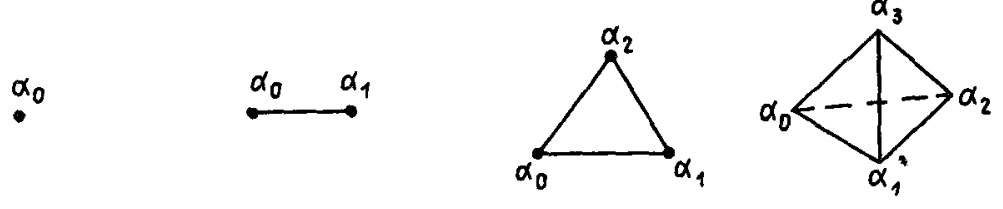
\includegraphics[width=0.80\textwidth]{figures/fig3_1.png}
  \figtitle{3.1}{(a) 0 维；(b) 1 维；(c) 2 维；(d) 3 维}
\end{figure}
% [Tutor Note: (1.1) 中的 $x^j$ 是重心坐标（上标记编号），不是幂；$\sum x^j=1$ 与 $x^j\ge0$ 一起说明 $\sigma^n$ 是其顶点的凸包而非线性张成。易错处：$n$ 维单形有 $n+1$ 个顶点，故 $n=0$ 时单形是一个点、$n=1$ 时是线段；写作 $\R^n$ 只是为了取坐标，单形本身与所在欧氏空间无关。]

单纯复形 $K$ 是单形的一个任意（有限或可数无限）族，满足以下性质：
1. 与族中每个单形一起，它的所有维数的所有面也都属于该族。
2. 族中任意两个相交的单形，或者重合（即同一个单形），或者恰好相交于一个公共面。

给出一个单纯复形的最方便方式，是指明它的顶点 $\alpha_0,\dots,\alpha_n,\dots$，以及这些顶点中确定该复形的单形的那些（有限）子集。
% [原文 p.42]
人们也可以考虑更一般的复形，它们不由单形组成，而由其他一般的凸多面体（更确切地说，多胞形）组成，但仍满足上面的条件 1 与 2；事实上我们将经常考虑这样的复形。然而容易证明，通过重分，这样的复形可以细化为单纯复形。在具体复形的同调研究中，常使用「合并」（consolidation）运算，即把适当的一组单形合并成凸多胞形。

\begin{remark}{}
除单纯复形外，\emph{立方复形}也很有意义。这种复形由各维的立方体 $I^n$ 组成（见图 3.2），按上述条件 1、2 的类比拼合成一个立方复形。每个单纯复形都可以经过适当的重分而取立方复形的形式，反之亦然。立方复形的便利之处在于 $I^{n+m}=I^n\times I^m$，于是立方复形的乘积仍是立方复形；它们的意义还来自 $\R^n$ 具有规则的正方体剖分（规则立方格）。在现代统计力学中，格模型理论里出现若干问题，涉及作为 $\R^n$ 的子流形在给定规则立方剖分下的像而出现的立方子复形。特别地，在 $n=3$ 的情形，必须找出曲面 $M^2$ 到 $\R^3$ 中规则立方格的映射的描述，其中 $M^2$ 被剖分成 2 维立方体（正方形），且映射保持这一结构。相应剖分的加细必须使得 $\R^3$ 中格的规则性得以保持。\footnote{「Novikov 问题」，最近由 N. P. Dolbilin, M. A. Stanko 与 M. I. Shtogrin 考虑。}
\end{remark}

\begin{figure}[htbp]
  \centering
  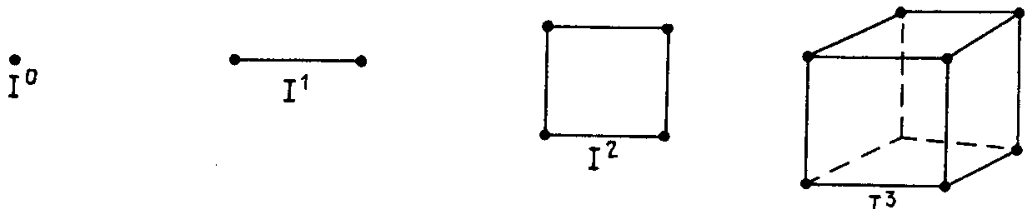
\includegraphics[width=0.74\textwidth]{figures/fig3_2.png}
  \figtitle{3.2}{(a) $I^0$；(b) $I^1$；(c) $I^2$；(d) $I^3$}
\end{figure}
% [Tutor Note: 原书 p.42 此处印作「subdivisions mu.st be such as」，其中 mu.st 显然是 must 的排印脱字，译文按 must 处理为「必须」。之所以要强调「加细必须保持格的规则性」，是因为任意加细都会破坏立方结构，使 $M^2$ 不再是被剖分成正方形的曲面。]

回到任意单纯（或凸多面体）复形 $K$，我们注意，若 $K$ 有限，即只由有限多个单形（或凸多胞形）组成，则可以为它定义第 1 章已提到的 \emph{Euler--Poincaré 示性数}：
\begin{equation}
  \chi(K)=\sum_{j\ge0}(-1)^j\gamma_j, \tag{1.3}
\end{equation}
% [原文 p.43]
其中 $\gamma_j$ 是 $K$ 的 $j$ 维单形（或 $j$ 维凸多胞形）的个数。若 $K$ 的每个单形的维数 $\le n$，且存在 $n$ 维单形，则称复形 $K$ 是 \emph{$n$ 维}的。$K$ 的 \emph{$m$ 维骨架}是由 $K$ 中所有维数 $\le m$ 的单形组成的子复形。
% [Tutor Note: (1.3) 里的 $\gamma_j$ 数的是「$j$ 维单形的个数」，不是 $j$ 维骨架的同调维数；$\chi$ 的同伦不变性（下文 Alexander 的结果）正说明它能由这些组合计数算出拓扑信息。注意 $(-1)^j$ 从 $j=0$ 起算，故点的 $\chi=1$、线段的 $\chi=1$、圆周的 $\chi=0$。]

给定两个单纯复形 $K$ 与 $K'$，若 $K$ 的每个单形都是 $K'$ 的有限多个单形之并，且 $K'$ 的单形都\emph{线性地}含于 $K$ 的单形之中，则称 $K'$ 是 $K$ 的一个\emph{重分}。任何单纯复形都有一个标准重分，称为\emph{重心重分}，它按如下方式归纳地定义：一个点（或 0 维单形）不作重分。一维单形 $\sigma^1=(\alpha_0,\alpha_1)$ 的重心重分通过在 $\sigma^1$ 的中心（中点）引入一个新顶点来完成，于是 $\sigma^1$ 变成由 3 个顶点与 2 个一维单形（棱）组成的复形。要对 $n$ 维单形 $\sigma^n\subset\R^n$ 作重心重分，先对其面作重心重分，然后在 $\sigma^n$ 的中心（重心）处引入又一个新顶点 $\alpha'\in\sigma^n$，并把所有形如 $(\beta_0,\dots,\beta_k,\alpha')$ 的单形（其中 $(\beta_0,\dots,\beta_k)$ 是 $\sigma^n$ 某个面的重心重分中的任意单形）都作为（重心重分的）新单形纳入。这些新单形的全体就构成 $\sigma^n$ 的重心重分（见图 3.3）。单纯复形的重心重分则通过对该复形的所有单形作重心重分而得到，并保证在两个或多个单形共有的面上，重分彼此一致。

\begin{figure}[htbp]
  \centering
  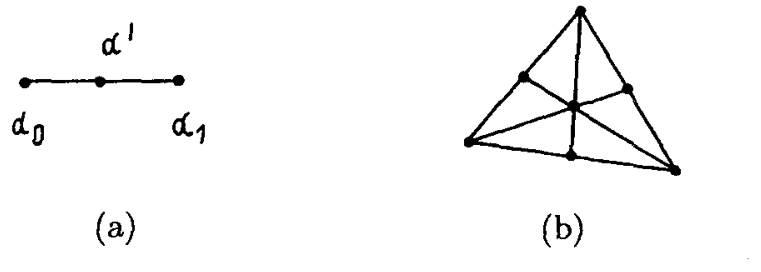
\includegraphics[width=0.50\textwidth]{figures/fig3_3.png}
  \figtitle{3.3}{单形的重心重分}
\end{figure}

\begin{definition*}{1.1}
两个单纯复形 $K_1$、$K_2$ 称为\emph{组合等价}的，若存在一个单纯复形 $K$，它同构于两者的某个重分。
\end{definition*}
% [Tutor Note: 组合等价是「在重分意义下的同构」，比单纯同构弱得多：任何复形都与它的重心重分组合等价，但两者作为复形一般不同构。Definition 1.1 只要求存在公共的加细 $K$，不要求 $K$ 是重心的；这一点在判断两个三角剖分是否等价时很关键。]

在拓扑学发展的某一阶段，当一切已知的拓扑不变量都用组合术语定义时，人们提出了后来称为 \emph{Hauptvermutung der Topologie}（拓扑学主猜想）的猜想，它当时被视为头等重要。这个猜想断言：任何两个同胚的复形都是组合等价的。用直接的初等方法证明了它在维数 $\le3$ 时成立（Moise 在
1950 年代——至少对流形如此），但后来发现它在维数 $\ge6$ 时不成立（Milnor，1960 年代初）。随后在 1970 年代末有人（Edwards）证明：任何「同调 3 球面」（即与 3 球面有相同同调的）3 维流形的二重悬挂，实际上同胚于 5 球面；并且由它得到的 $S^5$ 的三角剖分确实与平凡剖分（即单形 $\sigma^6$ 的边界）组合不等价。\footnote{Freedman 与 Donaldson（1980 年代初）的结果表明，Hauptvermutung 对 4 维流形也不成立。}
% [原文 p.44]

不管 Hauptvermutung 对具体空间成立与否，那些只依赖组合结构的最简单的拓扑不变量——例如 Euler--Poincaré 示性数与同调群（见下文）——不仅在自同胚下不变，甚至在同伦等价下也不变（Alexander，1920 年代）。（看来这正是同伦等价这一概念的来源。）更深的不变量——「Pontryagin 类」在闭链上的积分（它由 Thom--Rohlin--Schwarz 定理获得组合定义）与「Reidemeister--Whitehead 挠」——最初也可以组合地定义。虽然人们早已知道（Pontryagin 类自 1950 年代中期起，Reidemeister--Whitehead 挠自 1930 年代起）这些量不是同伦不变量，但结果表明它们至少是拓扑不变量，即在自同胚下不变（Pontryagin 类由 Novikov 在 1960 年代中期证得，Reidemeister--Whitehead 挠由 Edwards 与 Chapman 在 1970 年代证得；注意 $n=3$ 时这可由上面提到的 Moise 1950 年代的定理推出）。Reidemeister--Whitehead 挠构成拓扑学中一个本质上自成一体的篇章。我们以后会回到与这个不变量相关的后续发展（发生在 1960 与 70 年代），这些发展已汇成一个独特而高度复杂的理论。1960 年代中期，Sullivan 勾勒了一个漂亮的理论，其推论是：只要群 $H_3(M;\Z)$ 没有 2-挠，Hauptvermutung 对单连通的 PL 流形 $M$ 成立。\footnote{在 Sullivan 工作的最初版本中，他对群 $H_3(M)$ 未加任何限制；上述要求的必要性出现于与 Browder 和 Novikov 的讨论（1967 年春）。Sullivan 理论的阐述至今（至少到 1994 年写作时）尚未在文献中出现。} Kirby 与 Siebenmann 发展了一套理论，完全澄清了维数 $n\ne4$ 的流形上 PL 结构与拓扑结构之间的关系。\footnote{R. C. Kirby 与 L. C. Siebenmann 的书 \emph{Foundational essays on topological manifolds, smoothings, and triangulations}（Princeton University Press, 1977, Annals of mathematics studies, no.~88）专门讨论这一理论。在该书中作者显然试图对 Sullivan 的理论给出独立的验证。然而书中有若干关键陈述，其证明需要 Sullivan 的结果。例如，在本书作者看来，第 268--296 页的证明似乎并未独立于对 Sullivan 某些结果的引用而完整。当然，重要的是这些基本结果应被完整严格地确立并发表。此处应指出，Sullivan 所勾勒理论的一些困难已被
其他拓扑学家克服；例如同伦论方面所需的一切结果都已由 Milgram 与 Madsen 在他们关于流形的分类空间、手术与配边的书（\emph{Classifying Spaces in Surgery and Cobordism of manifolds}, University Press, 1979, Annals of mathematics studies, no.~92）中确立。该工作使用了若干 1967 年时尚未发展出来的技术工具与想法。}

% [原文 p.45]
任何情形下，对每个 $n\ge5$，闭的、光滑或分片线性（PL）流形的自同胚类总共只有有限多个（Novikov，1960 年代中期，单连通情形）。更详细的结果（属于 1960 年代末与 1970 年代）将在第 4 章 §5 末尾指出。
% [Tutor Note: 这一段是全书对「三角剖分是否拓扑不变」这一问题最集中的交代：$\chi$ 与同调群连纯组合定义都不怕（它们甚至同伦不变），而 Pontryagin 类与 Reidemeister--Whitehead 挠可组合定义却是拓扑不变量而非同伦不变量，二者的「层次」差别正是手术理论的出发点。Edwards 的二重悬挂例子说明：同胚的复形未必组合等价，故 Hauptvermutung 在 $\ge6$ 维失效并不与 $\chi$ 的不变性矛盾。]

回到单纯复形初等理论的阐述，我们把单形之间的\emph{映射} $\sigma_1^n\to\sigma_2^m$ 定义为把 $\sigma_1^n$ 的顶点映到 $\sigma_2^m$ 的顶点、并线性地延拓到整个 $\sigma_1^n$ 的任意映射。复形的\emph{单纯映射} $f:K_1\to K_2$ 是限制在每个单形上都是单形映射的映射；因此复形之间的单纯映射也由 $K_1$ 的顶点 $\alpha_j$ 的像 $f(\alpha_j)=\beta_j$ 决定，其中 $\beta_j$ 是 $K_2$ 的顶点。\emph{分片线性}（PL）\emph{映射} $K_1\to K_2$ 是指在 $K_1$ 与 $K_2$ 的某对适当重分 $\bar K_1$、$\bar K_2$ 之间为单纯映射的映射（重分不必是重心的）。

相当直接的「单纯逼近定理」断言：复形间的每个连续映射 $f:K_1\to K_2$ 都可以被 $K_1$ 与 $K_2$ 的适当重分的 PL 映射 $g:\bar K_1\to\bar K_2$ 任意接近地逼近，且 $g$ 同伦于 $f$。

有时使用这个定理的一个变体：给定一如前的任意映射 $f:K_1\to K_2$，存在单纯映射 $g:\bar K_1\to K_2$，此时只对 $K_1$ 取某个重分；$g$ 不必再接近 $f$，但它通过一个同伦与 $f$ 同伦，且该同伦过程中每个像点的移动都限制在 $K_2$ 的单个单形之内。
% [Tutor Note: 单纯逼近定理的两个版本用途不同：第一版给出「同伦于 $f$ 且接近 $f$」的 PL 映射，用于把连续映射换成组合映射；第二版放弃「接近」，只保留「同伦于 $f$ 且像点移动不跨越 $K_2$ 的单个单形」，用于追踪 $f$ 在某个单形上的行为（例如证明单纯映射与同伦类的关系）。别把两版的条件记混。]

\begin{definition*}{1.2}
若经过一列重心重分之后，单纯复形 $K$ 的每个单形的\emph{组合邻域}（即由以该单形为面的单形连同它们的边界组成的复形）都是组合等价于 $\sigma^n$ 的复形，则称 $K$ 是 \emph{$n$ 维 PL 流形}。
\end{definition*}

$n$ 维 PL 流形称为\emph{可定向}的，若它的 $n$ 维单形可以全都如此定向，使得在每个 $(n-1)$ 维单形上，由以它为公共面的两个 $n$ 维单形的定向所诱导的定向相反。把一个（可定向）PL 流形的 $n$ 维单形定向以使这一准则得到满足的每种具体方式，称为该 PL 流形的一个\emph{定向}。
% [Tutor Note: Definition 1.2 里「经过一列重心重分之后」这个限定不能省：单形上某点的链环（组合邻域）在原始剖分下可能只是一个锥而并非球面，重心重分把这种病态「抹平」。也正因如此，PL 流形不等于「每个单形的邻域都像球面的复形」——后者是更强的、一般三角剖分不满足的条件。]

当然，每个 PL 流形都是拓扑流形。然而并非拓扑流形的每个三角剖分都给出作为 PL 流形的单纯复形：我们已经提到 Edwards 的定理（1970 年代），它说的是：由任何同调 3 球面 $M^3$（即满足 $H_1=H_2=0$ 但 $\pi_1\ne0$ 的 3 维流形）的二重悬挂 $\Sigma\Sigma M^3$ 得到的球面 $S^5$ 的三角剖分，与 $\sigma^5$ 组合不等价，然而 $\Sigma\Sigma M^3\cong S^5$（其中 $\cong$ 表示「同胚于」）。

% [原文 p.46]

\begin{figure}[htbp]
  \centering
  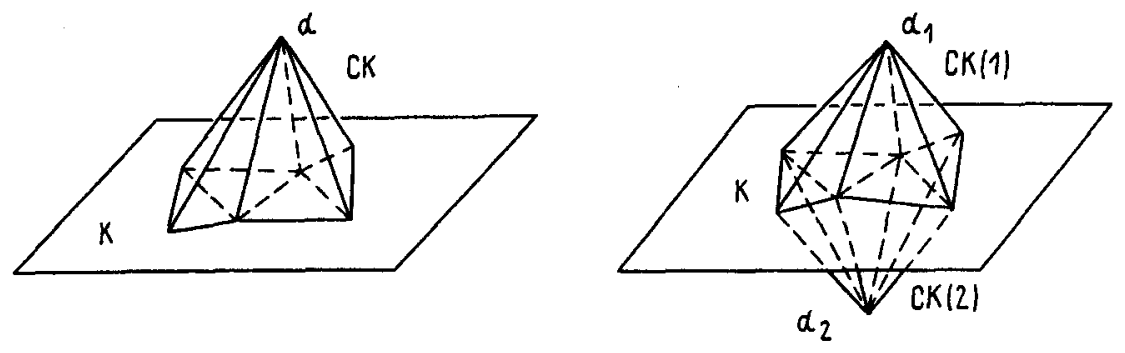
\includegraphics[width=0.80\textwidth]{figures/fig3_4.png}
  \figtitle{3.4}{(a) $K$ 上的锥；(b) 悬挂 $\Sigma K=(CK)_1\cup(CK)_2$}
\end{figure}

现在我们来定义其中一些术语。单纯复形 $K$ 上的\emph{锥}，记作 $CK$，是把 $K$ 的每一点用一条线段与 $K$ 外的一个新顶点 $\alpha$ 相连所得的复形；它的三角剖分按显然的方式给出，使 $CK$ 成为单纯复形（见图 3.4(a)）。$K$ 的\emph{悬挂} $\Sigma K$ 则是 $K$ 上两个锥把公共底 $K$ 等同起来的并：
\begin{equation}
  \Sigma K=(CK)_1\cup_K(CK)_2. \tag{1.4}
\end{equation}
悬挂于是可以按显然的方式三角剖分（见图 3.4(b)）。

\begin{figure}[htbp]
  \centering
  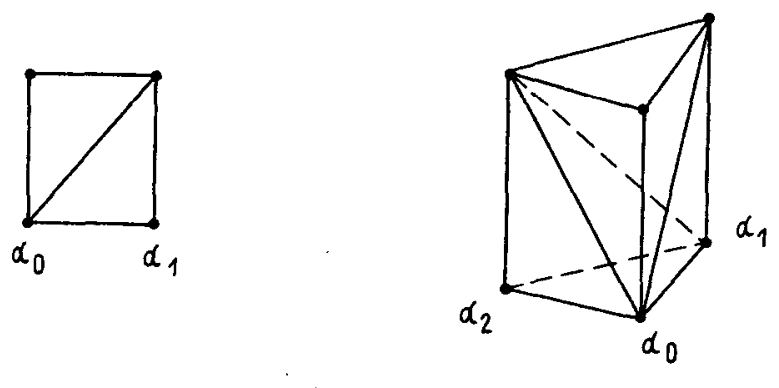
\includegraphics[width=0.46\textwidth]{figures/fig3_5.png}
  \figtitle{3.5}{单形上柱体的重分}
\end{figure}
% [Tutor Note: (1.4) 中 $\cup_K$ 表示沿公共底 $K$ 粘合，两个锥各带一个顶点，故 $\Sigma K$ 比 $K$ 高出一维；这与第 2 章 §1 的悬挂是同一构造。图 3.5 画的是 $K\times I$ 的重分（正方形剖成两三角形、立方体剖成若干四面体），这是把乘积做成单纯复形的标准手段；与之相关的一句说明在第 3 章 §1 之后（见 p.47 顶端括注）。]

第 2 章 §1 中引入的拓扑空间的基本运算，即楔和 $K_1\vee K_2$、（单纯）映射柱 $C_f$，$f:A\to K_2$、$A\subset K_1$，以及乘积 $K_1\times K_2$，在每种运算之后再作某个（标准的）重分，就都仍落在单纯复形类中。
% CHUNK ch03a DONE
